\documentclass[12pt,letterpaper]{article}
 
\usepackage[plain, cm, myheadings]{fullpage}
\usepackage{afterpage}
\usepackage{setspace}
\usepackage{xspace}
\usepackage{verbatim}
\usepackage{graphicx}
\usepackage{color}
\usepackage{lscape}
\usepackage{amsmath}
\usepackage{array}
\usepackage{multirow}
 
\pagenumbering{arabic}
 
\setlength{\parindent}{0em}
\setlength{\parskip}{0.75ex plus0.25ex minus0.25ex}
\setlength{\extrarowheight}{3pt}

\newcommand{\subscript}[1]{\ensuremath{_{\text{\scriptsize #1}}}}
\newcommand{\Ka}{K\subscript{a}\xspace}

\begin{document}

\markright{National Center for Atmospheric Research}

\title{HIAPER Cloud Radar Transceiver Design}
\author{Gordon Farquharson\\
National Center for Atmospheric Research\\
Boulder, CO}
\maketitle

\section{Introduction}

This document details the design for the ground-based two-antenna
cloud radar prototype which will become the HIAPER Cloud Radar
(HCR). The design requirements are described in
Section~\ref{sec:design_requirements}. Section~\ref{sec:overview}
presents an overview of the transceiver design including the
transceiver block diagram. Section~\ref{sec:if_selection} outlines the
decisions made in selecting the second stage intermediate frequency in
the transceiver. The design and simulation of the waveform generator
is presented in Section~\ref{sec:waveform_generator}. The description
of the up- and down-conversion electronics is presented in
Sections~\ref{sec:upconversion} and \ref{sec:receiver}
respectively. Section~\ref{sec:calibration} presents the calibration
measurements that will be made in the system, and
Section~\ref{sec:system_performance} summarizes the system performance
with this transceiver design.

\section{Design Requirements}
\label{sec:design_requirements}

\textit{This section is not complete.}

The receiver bandwidth is determined by the minimum range resolution
specification (30 meters). For a pulse width of 200~ns, the bandwidth
is 5~MHz. However, the phase~B HIAPER system will use pulse
compression to increase the average transmit power and therefore the
sensitivity of the system. To achieve low range side lobes with a
pulse compression system, the spectrum of the transmitted pulse will
be shaped, resulting in an increase in required receiver bandwidth for
a given range resolution. To accommodate this increase in bandwidth,
all of the receiver components for the ground-based radar and the
phase~A HIAPER radar, are specified for a minimum 20~MHz pass band to
accommodate lower range resolutions. The sensitivity of the system
will be optimized to the pulse length used by digitally filtering the
received signal to desired signal bandwidth after digitization.

Other transceiver specifications:
\begin{itemize}
\item Transmit pulse width that ranges from 200~ns to 2~$\mu$s (30 to
  300 meter range resolution, 500~kHz to 5~MHz bandwidth) at a PRF
  between 1 to 20~kHz.
\item Must be able to generate frequency modulated pulses to implement
  pulse compression.
\item Must be able to predistort pulse to compensate for amplitude and
  phase variations in the transceiver electronics.
\item Must support frequency modulated pulses of up to 20~MHz in
  bandwidth.
\item Radar must have 80~dB of dynamic range (includes
  post-processing).
\item Must not interfere with aircraft systems including
  communications band (108 to 137~MHz).
\end{itemize}

\section{Transceiver Overview}
\label{sec:overview}

A block diagram of the ground-based transceiver (single-wavelength,
single-polarization transceiver) is shown in
Figure~\ref{fig:ground_system}. The transceiver consists of three main
sections: the electronics to up-convert the transmitted signal from
the intermediate frequency to W-band; the electronics to down-convert
the W-band received signal to the intermediate frequency; and a
down-conversion channel to sample the transmitted waveform. The
transceiver uses a two-stage up- and down-conversion super-heterodyne
design. The first stage intermediate frequency is 156.25~MHz and the
second stage intermediate frequency is 1406.25~MHz. Two antennas are
used in this system to achieve isolation between the transmitter and
receiver. Nominal signal levels are shown in
Figure~\ref{fig:ground_system} in a bolder font next to the signal
lines.

There are four connections between the transceiver and the data
system: the signal from the waveform generator; the 125~MHz system
clock; and two intermediate frequency signals from the receiver
channel and the transmit sample channel. Although the waveform
generator is contained on the Pentek Model 7142 transceiver card, the
waveform generator is considered part of the transceiver and is
discussed in this document. The document does not discuss the
digitizers in detail, but does present an analysis for the
requirements of the receiver noise level at the input to the
digitizers. The system clock connects directly to the Pentek card.

\afterpage{
  \begin{landscape}
    \begin{figure}[p]
      \centering
      \includegraphics[scale=0.6]{ground_system-no_border.eps}
      \caption{Transceiver block diagram.}
      \label{fig:ground_system}
    \end{figure}
  \end{landscape}
}

\section{Intermediate Frequency}
\label{sec:if_selection}

The intermediate frequency and analog to digital sampling rate
selected for the radar are 156.25~MHz and 125~MS/s respectively. This
section describes the factors that resulted in these selections. Other
intermediate frequency and sampling frequency combinations are
discussed in Section~\ref{sec:waveform_generator} after the waveform
generator design has been presented.

The HCR will use pulse compression to increase the sensitivity of the
system. Since pulse compression waveforms used in radars with range
resolutions of tens of meters have bandwidths in the megahertz to tens
of megahertz range, the intermediate frequency must be sufficiently
high to provide enough bandwidth for sufficient suppression of
unwanted harmonics and mixer products. Therefore, intermediate
frequencies in the tens to hundreds of megahertz are desirable.

The HCR will be used in an airborne environment in which the VHF
aviation communications band (Airband, 108 to 137 MHz) exists. To
eliminate interference in the radar signals from aircraft
communications, the HCR intermediate frequency must be chosen outside
this band. In addition, the intermediate frequency must be high enough
to support wide bandwidth (up to 20 MHz) signals, and if possible,
when sampled by the digitizer, alias to the frequency that is equal to
the sampling frequency divided by four. This latter requirement allows
for the implementation of the $f_s/4$ demodulation scheme for
narrow-band signals which simplifies the digital demodulation
logic. However, the intermediate frequency is limited by the
technology available to generate an arbitrary wide bandwidth waveform,
and the ability to suppress undesired mixer products that result from
the frequency up- and down-conversion process.

An intermediate frequency of 156.25~MHz, in conjunction with a
sampling frequency of 125~MS/s, satisfies the $f_s/4$ demodulation
scheme for narrow-band signals. A signal centered at 156.25~MHz will
alias to 31.25~MHz when sampled at a rate of 125~MS/s, and 31.25~MHz
is one quarter of 125~MHz as required.

\section{Waveform Generator}
\label{sec:waveform_generator}

The advent spread spectrum coding schemes such as CDMA, TDMA, and OFDM
in communications has provided a demand for wide-bandwidth high-speed
digital to analog converters (DACs) that include digital up-conversion
circuitry. These up-converting DACs are ideal for generating pulse
compression waveforms with an arbitrary amplitude taper and frequency
modulation that allows one to predistort a pulse compression waveform
in amplitude and phase to compensate for amplitude and phase
distortions due to microwave components in the transceiver. Several
vendors have incorporated these DACs into transceiver cards which is
appealing because these cards have both a DAC for generating the
waveform for transmission, and digital down-conversion (DDC)
electronics to digitize received signals. Based on a survey of
available cards, the best choice in terms of size and functionality
appears to be the Pentek Model 7142 which has a single channel 16-bit
500~MS/s interpolating and up-converting DAC (Texas Instruments
DAC5686/7), and four 14-bit 125~MHz analog to digital converters
(Linear Technologies LTC2255). The card is in the PMC form factor
which can be mounted on various other carrier cards sold by Pentek
including CompactPCI.

In addition to the features mentioned above, the Model 7142 is
appealing because it is similar to the Model 7140 that the EOL wind
profilers will use. Thus, software developed for one system could be
reused in the other. The differences between the cards are that the
7142 provides a Xilinx Virtex-4 FPGA as opposed to GC4016 Gray Chips
and a Xilinx Virtex-II FPGA to implement the DDC, and the 7142 only
routes one of the two DAC5686/7 analog outputs to a connector on the
front panel of the board. This difference means that the DAC5686/7 can
only be used in the single channel or quadrature modulation mode, and
cannot be used in the single-sideband mode that was originally
envisioned in the HCR Preliminary Design Review document.

This section presents simulations that show that the performance of
the DAC5687 used on the Pentek Model 7142 is suitable for use in the
HIAPER Cloud Radar. Section~\ref{sec:dac_distortions} provides an
introduction to distortions present in the output of
DACs. Section~\ref{sec:dac_analysis} details how the waveform will be
synthesized with this device, and the results of simulations of
waveforms with the the device.

\subsection{Distortions in DAC-Generated Signals}
\label{sec:dac_distortions}

Digital to analog converters do not produce a perfect analog
representation of the digital input signal. The output signal is
corrupted through the non-linear mapping of the input codes to output
codes, and clock-related spurious signals. The effect of these
distortions must be understood in the application in which the DAC is
used. The theory of digital to analog converters is well documented
(e.g.~\cite{slaa013}), and thus, this section only provides a brief
overview of the distortions considered in this design study.

\subsubsection{Harmonic Signals}
\label{sec:harmonic_spurious}

The output code is a combination of the input code, the integral
non-linearity error, the gain error, and the offset error, and is
given by
\begin{equation}
  O(I)=\left(I+\epsilon_\text{lsb}^I\right)\frac{F-\epsilon_\text{g}}{F}+\epsilon_\text{offset}
\end{equation}
where $I$ is the input code, $O(I)$ is the output code,
$\epsilon_\text{lsb}^I$ is the integral non-linearity error associated
with the input code, $F$ is the full scale code, $\epsilon_\text{g}$
is the gain error, and $\epsilon_\text{offset}$ is the offset
error. The definition of each of these terms is defined in detail in
various texts and will not be repeated here. The values are typically
listed in the DAC data sheet.

The non linearity of the conversion from the input code to the output
voltage generates harmonics of the output signal. An example spectrum
of a DAC signal is shown in Figure~\ref{fig:dac_harmonics}. In this
example, the output signal is centered at a frequency of 25~MHz, and
the output sample rate from the DAC is 120~MHz. The top part of the
signal shows the result of the non-linear conversion which generates
harmonics of the desired output signal at integer multiples of the
output signal frequency. The desired output signal is drawn in black,
and the first eight harmonics are drawn in various colors and are
labeled with their harmonic number. The signals in the negative part
of the spectrum are drawn with dashed lines. Since the output waveform
is a continuous representation of a sampled process, the harmonics
outside the Nyquist zone ($-$60 to 60~MHz) aliases into the Nyquist
zone, and the result is sketched in the bottom part of the figure. In
this example, the desired signal is corrupted by the forth and sixth
harmonics. In general, the frequency of the aliased harmonics is
determined by the frequency of the desired signal and the output DAC
sampling rate. The level of the harmonics is determined by the
non-linear error in the conversion processes which in general is
different for each DAC.

\begin{figure}[htbp]
  \centering
  \includegraphics[scale=0.9]{dac_spectrum.eps}
  \caption{The top part of the figure shows the harmonics of an output
    signal centered at 25 ~MHz. The bottom part of the figures shows
    how these harmonics are mapped into the Nyquist range.}
  \label{fig:dac_harmonics}
\end{figure}

\subsubsection{Non-Harmonic Spurious Signals}
\label{sec:non-harmonic_spurious}

Many high speed DACs are able to interpolate between input samples to
produce an output rate that is higher than the input rate. Typical
interpolation factors are 2, 4, 8, and 16. Interpolation provides high
output sample rates without the need for an equivalent input sample
rate, and separates the desired signal from images in adjacent Nyquist
zones. However, the subharmonic frequencies of the DAC clock that are
used for the interpolation filters, mix with the DAC clock due to
imperfect isolation between the internal digital logic and DAC clock
circuits, and create images of the desired signal. The amplitude and
location of these spurious signals in the frequency spectrum depend on
the frequency of the desired output signal, the DAC output rate, and
the amount of interpolation. In many situations, these spurious
signals are the dominant signals that exist close to the desired
signal frequency, and therefore can be hard to filter.

\subsection{Waveform Generator Implementation and Analysis}
\label{sec:dac_analysis}

The intermediate frequency and sampling rate are 156.25~MHz and
125~MS/s respectively. The 156.25~MHz signal will be generated by the
DA5687 internal digital up-conversion circuitry. A functional block
diagram of the DAC5687 in the \texttt{X4L/FMIX/CMIX} mode and with
\texttt{cm\_mode(3:0) <= 1001} (\texttt{CONFIG2} register) is shown in
Figure~\ref{fig:dac5687-x4l}. The real $I[n]$ and imaginary $Q[n]$
parts of a base band signal are the input to the DAC5687. The input
sampling rate is 125~MS/s. These signals are interpolated up to a
sampling rate $f_{s_1}$ of 250~MS/s ($I_\text{x2}[n]$ and
$Q_\text{x2}[n]$). The fine mixer stage of the DAC5687 uses an NCO
running at 250~MS/s to generate a Hilbert transform pair
($m_\text{x2}[n]$ and $m_{\text{x2}h}[n]$) centered at a frequency
$f_{c_1}$ of 31.25~MHz at the output of the fine mixer stage (see
DAC5687 datasheet, p.~37 in the section on the fine mixer or p.~68).
\begin{equation}
  \begin{aligned}
    m_\text{x2}[n] &= I_\text{x2}[n]\cos\left(2\pi\frac{f_{c_1}}{f_{s_1}}n\right)-Q_\text{x2}[n]\sin\left(2\pi\frac{f_{c_1}}{f_{s_1}}n\right) \\
    m_{\text{x2}h}[n] &= I_\text{x2}[n]\sin\left(2\pi\frac{f_{c_1}}{f_{s_1}}n\right)+Q_\text{x2}[n]\cos\left(2\pi\frac{f_{c_1}}{f_{s_1}}n\right)
  \end{aligned}
\end{equation}
This Hilbert transform pair of signals is then interpolated to a
sampling rate $f_{s_2}$ of 500~MS/s ($m_\text{x4}[n]$ and
$m_{\text{x4}h}[n]$), and these signals become the input to the course
mixing stage. The course mixing stage in the DAC5687 is limited to
frequency up-converting signals by either $f_{s_2}/2$ or
$f_{s_2}/4$. In this application, the $f_{s_2}/4$ mode is used to
frequency up-convert the Hilbert transform pair to single sideband
signal centered at 156.25~MHz. The inverse sinc filter $(x/\sin x)$ is
used to compensate for gain changes across the band due to the
zero-order hold output of the DAC. The input to the digital to analog
converter (DAC~A) in the DAC5687 is
\begin{align}
  y[n] & = m_\text{x4}[n]\cos\left(2\pi\frac{f_{c_2}}{f_{s_2}}n\right)-m_{\text{x4}h}[n]\sin\left(2\pi\frac{f_{c_2}}{f_{s_2}}n\right) \label{eq:dac_input} \\
  & = I_\text{x4}[n]\cos\left(2\pi\frac{f_{c_1}+f_{c_2}}{f_{s_2}}n\right) - Q_\text{x4}[n]\sin\left(2\pi\frac{f_{c_1}+f_{c_2}}{f_{s_2}}n\right)
\end{align}
where $f_{c_1}+f_{c_2}=$156.25~MHz, and $f_{s_2}=$500~MS/s. This
signal is a single sideband signal (upper sideband) centered at
156.25~MHz.

The course mixing stage output sequence is selected by
bits \texttt{cm\_mode(3:0)} in the \texttt{CONFIG2} register. With
$f_{c_2}=125$~MHz and $f_{s_2}=500$~MS/s, Equation~\ref{eq:dac_input}
simplifies to
\begin{equation}
  y[n] = m_\text{x4}[n]\cos\left(2\pi n/4\right)-m_{\text{x4}h}[n]\sin\left(2\pi n/4\right)
\end{equation}
which, for $n=0,1,2,3,4,5,\ldots,$
\begin{equation*}
  y[n]=m_\text{x4}[0],\,-m_{\text{x4}h}[1],\,-m_\text{x4}[2],\,m_{\text{x4}h}[3],\,m_\text{x4}[4],\,-m_{\text{x4}h}[5],\,\ldots
\end{equation*}
The course mixing output sequence sequence for this application is
found by comparing the sequence above with the sequences found in
Table~10 of the DAC5687 datasheet (p.~38). In this case, the sequence
corresponds to the sequence associated with the output from DAC~A with
\texttt{cm\_mode(3:0) <= 1001}.

\begin{figure}[htbp]
  \centering
  \includegraphics[scale=0.65]{dac5687-x4l.eps}
  \caption{DAC5687 X4L operating mode. In- and quadrature-phase
    samples are interpolated to twice the input sampling rate, and then
    frequency up-converted to an intermediate frequency (31.25~MHz) by
    the fine mixer stage. The result it a Hilbert transform pair which
    is interpolated by a factor of two again, and then frequency
    up-converted to the final intermediate frequency (156.25~MHz).}
  \label{fig:dac5687-x4l}
\end{figure}

\textbf{This document does not yet describe how to set up the FIR
filters in the DAC5687 or any of ther other registers to configure the
DAC for the mode of operation discussed.}

As described in Section~\ref{sec:non-harmonic_spurious}, the
interpolation provided by the DAC5687 causes non-harmonic spurious
signals in the output. Table~\ref{tab:spurious} lists the frequency
and worst-case level of these spurious signals. The signals at 93.75
and 218.75~MHz are both 62.5~MHz from 156.25~MHz, and will need to be
suppressed by around 30~dB. These signals will define the requirements
for the bandpass filter at the output of the DAC.

\begin{table}[htbp]
  \centering
  \caption{DAC spurious output signals due to clock related mixing
    internal to the DAC.}
  \label{tab:spurious}
  \vspace{0.5em}
  \begin{tabular}{|l|c|c|}
    \hline
    \multicolumn{1}{|c|}{\textbf{Spurious}} & \textbf{Frequency} & \textbf{Level} \\
    \hline
    & \multicolumn{1}{c|}{MHz} & \multicolumn{1}{c|}{dBc} \\
    \hline
    $f_\text{SIG}+\dfrac{f_\text{DAC}}{4}$  & 281.25 & $-$41 \\
    \hline
    $f_\text{SIG}-\dfrac{3}{4}f_\text{DAC}$ & 218.75 & $-$41 \\
    \hline
    $f_\text{SIG}-\dfrac{f_\text{DAC}}{2}$ & 93.75 & $-$47 \\
    \hline
    $f_\text{SIG}-\dfrac{f_\text{DAC}}{4}$ & 31.25 & $-$41 \\
    \hline
  \end{tabular}
\end{table}

The closest harmonically related signals generated by the DAC were
calculated through a simulation that used the integral non linearity
error data provided by Texas Instruments, and the gain and offset
error from data sheet for the DAC5687. The simulated output waveform
and spectrum of the DAC, without the inverse sinc compensation, is
shown in Figure~\ref{fig:spectrum_images}. A DC component to the
spectrum is predicted due to the offset error of the
DAC. Figure~\ref{fig:spectrum_harmonics} shows the same spectrum over
a reduced frequency range, and identifies the locations and levels of
the first 15 harmonics between 0 to 250~MHz. These harmonics are also
tabulated in Table~\ref{tab:harmonics}. The closest harmonics occur at
31.25~MHz from the intermediate frequency signal at 125 and 187.5~MHz,
but are more than 90~dB below the carrier.

The simulation did not consider clock jitter or the effects of only
using a 32-bit NCO in the first stage of the up-conversion. However,
if the resolution of the NCO causes the harmonics to increase
significantly, the input signal can be changed to the Hilbert
transform pair of signals sampled at 125~MS/s and the fine mixer stage
bypassed.

\begin{figure}[htbp]
  \centering
  \includegraphics[scale=0.8]{spectrum-images.eps}
  \caption{The top part of the figures shows the output waveform from
    the DAC of the signal at 156.25~MHz. The bottom part of the spectrum
    of the output signal from $-$1500 to 1500~MHz.}
  \label{fig:spectrum_images}
\end{figure}

\begin{figure}[htbp]
  \centering
  \includegraphics[scale=0.8]{spectrum-harmonics.eps}
  \caption{The spectrum of the output waveform between 0 and 250~MHz
    shown in Figure~\ref{fig:spectrum_images}. The first 15 harmonics of
    the output signal are shown.}
  \label{fig:spectrum_harmonics}
\end{figure}

\begin{table}[htbp]
  \renewcommand{\multirowsetup}{\centering}
  \centering
  \caption{DAC harmonics due to the DAC non linear conversion}
  \label{tab:harmonics}
  \vspace{0.5em}
  \begin{tabular}{|r|r|r|r|}
    \hline
    \multirow{2}{*}{\textbf{Harmonic}} & \multirow{2}{*}{\textbf{Frequency}} & \multicolumn{2}{c|}{\textbf{Aliased}} \\
    \cline{3-4}
    & & \multicolumn{1}{c|}{$\mathbf{+}$} & \multicolumn{1}{c|}{$\mathbf{-}$} \\
    \hline
    & \multicolumn{1}{|c|}{MHz} & \multicolumn{1}{c|}{MHz} & \multicolumn{1}{c|}{MHz} \\
    \hline \hline
    1 & $\pm$156.25 & 156.25 & $-$156.25 \\
    \hline
    2 & $\pm$312.50 & $-$187.50 & \textbf{187.50} \\
    \hline
    3 & $\pm$468.75 & $-$31.25 & 31.25 \\
    \hline
    4 & $\pm$625.00 & \textbf{125.00} & $-$125.00 \\
    \hline
    5 & $\pm$781.25 & $-$218.75 & 218.75 \\
    \hline
    6 & $\pm$937.25 & $-$62.50 & 62.50 \\
    \hline
    7 & $\pm$1093.75 & 93.75 & $-$93.75 \\
    \hline
    8 & $\pm$1250.00 & 250.00 & $-$250.00 \\
    \hline
    9 & $\pm$1406.25 & $-$93.75 & 93.75 \\
    \hline
    10 & $\pm$1562.50 & 62.50 & $-$62.50 \\
    \hline
    11 & $\pm$1718.75 & 218.75 & $-$218.75 \\
    \hline
    12 & $\pm$1875.00 & $-$125.00 & 125.00 \\
    \hline
    13 & $\pm$2031.25 & 31.25 & $-$31.25 \\
    \hline
    14 & $\pm$2187.50 & \textbf{187.50} & $-$187.50 \\
    \hline
    15 & $\pm$2343.75 & $-$156.25 & \textbf{156.25} \\
    \hline
  \end{tabular}
\end{table}

\section{Up-conversion Electronics}
\label{sec:upconversion}

The up-conversion electronics in the transceiver are configured in a
two-stage super-heterodyne
configuration. Figure~\ref{fig:tx_upconversion} shows a frequency
domain representation of the signals implemented in the
transceiver. The signal at the output of the waveform generator
(156.25~MHz) is up converted to 1406.25~MHz using a single sideband
modulator and then filtered to suppress the image frequency lower side
band signal (1093.75~MHz). The signal at 1406.25 GHz is then
up-converted to W-band (94.40625~GHz) with a W-band single-sideband
modulator, and filtered before transmission. The choice of the local
oscillator frequencies are such that they are integer multiples of the
125~MHz master oscillator.

\afterpage{
  \begin{landscape}
    \begin{figure}[p]
      \centering
      \includegraphics[scale=0.7]{tx_upconversion.eps}
      \caption{Output of the source and each filter and mixer stage.}
      \label{fig:tx_upconversion}
    \end{figure}
  \end{landscape}
}

\subsection{Spectrum Analysis}

The filter at the output of the waveform generator must suppress the
spurious signals that are generated by the waveform generator. The
transmitter spurious output level is specified to be less than 70~dB
which means that we should suppress the spurious and harmonically
generated signal from the waveform generator by at least this much.

From the results of the simulations of the waveform generator
(Table~\ref{tab:spurious}), the suppression at 93.75~MHz must be
greater than 23~dB and at 218.25~MHz must be greater than 29~dB to
suppress the non harmonically-generated spurious signal by greater
than 70~dB. The results in Figure~\ref{fig:spectrum_harmonics} show
that all harmonically generated signals are lower than 80~dB below the
carrier so little to no suppression is required at these frequencies.

Two designs were investigated for the IF bandpass filter using the
Lorch Microwave web-based filter selection
tool. Table~\ref{tab:lorch_filter_suppresion} show that both designs
easily exceed the suppression requirements. These numbers were
confirmed by contacting Lorch Microwave.

\begin{table}[htbp]
  \renewcommand{\multirowsetup}{\centering}
  \centering
  \caption{First stage intermediate frequency band pass filter
  characteristics.}
  \label{tab:lorch_filter_suppresion}
  \vspace{0.5em}
  \begin{tabular}{|c|c|c|}
    \hline
    Frequency & Filter 1 (4BP8-156.25/R20-S) & Filter 2 (4BC-156.25/R20-S) \\
    MHz & dB & dB \\
    \hline
    93.75  & 75.9 & 38.2 \\
    125.00  & 35.1 & 20.0 \\
    187.5   & 15.1 & 23.3 \\
    218.75  & 31.6 & 45.39 \\
    \hline
  \end{tabular}
\end{table}

The group delay at 146.25, 156.25, and 166.25~MHz for each filter is
respectively, 64.5, 36.4, and 43.9~ns, and 58.7, 38.1,
61.6~ns. Therefore, the maximum phase distortion due to the group
delay through the filters are 3.74 and 4.28 degrees. This phase change
can be compensated for by predistorting the transmitted signal to give
good range side lobe performance for pulse compression waveforms. This
analysis shows that a filter is feasible for this transceiver design.

The 156.25~MHz signal is mixed up to 1406.25~MHz using an local
oscillator of 1250~MHz ($10\times125$~MHz). The bandwidth of the
transmitted signal is up to 20~MHz (146.25 to 166.25~MHz). All mixer
products calculated from the first six harmonics of the intermediate
frequency and local oscillator fall outside the intermediate frequency
band. The closest mixer product to the second stage intermediate
frequency band results from the second harmonic of the local
oscillator (2500~MHz) and the sixth harmonic of the intermediate
frequency (877.5 to 997.5~MHz) and occurs at 1502.5 to 1622.5~MHz
which is 96.25~MHz from the second stage intermediate frequency band.

The second stage intermediate frequency filter must suppress the local
oscillator signal (1250~MHz), the lower sideband signal (centered at
1093.75~MHz, see Figure~\ref{fig:tx_upconversion}), and the eighth
order harmonic (1502.5 to 1622.5~MHz). The single sideband modulator
(Miteq SDM0102LC1CDC) will provide typically 20~dB suppression of the
lower sideband, and typically 30~dB suppression of the local
oscillator. The local oscillator signal is 156.25 MHz from the desired
signal and will not mix back into the receiver band, but the image
signal will. Therefore, to achieve 70~dB suppression of the image
signal, the filter must suppress the image (1083.75 to 1103.75~MHz) by
a minimum of 50~dB. The Lorch Microwave web-based filter selection
tool was shows that a suppression of greater than 84~dB can be
achieved with the 4BP7-1406.25/R50-S discrete filter, which is more
than sufficient. The local oscillator signal will be suppressed by
54.7~dB with this filter. Therefore, the second-stage intermediate
frequency image band will be suppressed by greater than 104~dB. The
eighth order harmonic will be suppressed by a minimum of 28.3~dB with
this filter.

The signal is mixed up to 94.40625~GHz using a local oscillator of
93~GHz ($744\times125$~MHz). All mixer products that result from the
first six harmonics of the second stage intermediate frequency and the
local oscillator lie outside the band of interest.

The 94.40625~GHz filter must suppress the 93~GHz local oscillator
signal and the image band (91.58375 to 91.91625~GHz, see
Figure~\ref{fig:tx_upconversion}). The W-band single-sideband
modulator (Farran Technology BMC-10-94-7-7 with side band filter) will
suppress the local oscillator and lower sideband by a minimum of
20~dB. The W-band pass filter (Millitech FIB-10-01000) has a minimum
suppression of 25~dB at 93 and 95~GHz. Therefore, the image band will
be suppressed by a total of more than 45~dB (see
Figure~\ref{fig:tx_upconversion}). Signals outside the transmitter
bandwidth will be further suppressed on transmission.

\subsection{Component Impedance Matching}

Although Millitech claims that the W-band filter (FIB-10-01000) can be
operated with any source and load VSWR, other filter manufacturer
vendors recommend that the maximum load VSWR be less than
1.5:1. Because the input VSWR of the EIKA driver amplifier (Farran
Technology FPA-10-16-19) is expected to be not better than 2.0:1, an
isolator (Millitech JFD-10-RI1SP) is used to improve the VSWR of load
seen by the filter.

The extended interaction klystron amplifier (EIKA) input VSWR can be
as high as 10.0:1. The maximum load VSWR recommended for the driver
amplifier is 2.0:1, so another isolator is used between the driver
amplifier and the EIKA.

The EIKA load VSWR must be less than 1.2:1 to achieve the specified
performance from the klystron. The directional coupler (Quinstar
Technology QJR-W40300) at the output of the EIKA has an maximum VSWR
of 1.1:1 which is sufficient to ensure good performance the EIKA. The
directional coupler also provides 70~dB of isolation between the
klystron and the antenna.

\subsection{Power Levels}

The nominal output power for the up-conversion electronics is 60.7~dBm
(1175 W). Due to imperfect matching between components, the output
power cannot be completely predicted because the input impedance seen
by a previous stage depends on the electrical distance between it and
the next component. Without simulation tools such as ADS, an accurate
estimate of the output power cannot be computed.

The output power analysis was computed using an output power from the
driver amplifier of 7.8~dBm which is 2.2~dB below the minimum
specified 1~dB compression point of the amplifier. After the isolator,
this power level is 7.0~dBm (5~mW). The EIKA typical drive power is +3
to +7~dBm (2 to 5~mW) and has an absolute maximum input power of
+10~dBm. Therefore, a 1~dB compression point of the driver amplifier
(+10~dBm) is sufficient to drive the amplifier, and provides some
degree of protection from over driving the EIKA.

The EIKA can operate with a load VSWR up to 2.0:1 without
damage. Therefore, the maximum reflected power for 1.7~kW output power
is 190~W. The directional coupler (Quinstar Technology QJR-W40300)
provides 30~dB of isolation between the antenna and the transmitter,
so that if the antenna were to transmit into a 0~dB return loss load,
the transmitter would see a maximum of 1.7~W reflected from the
antenna through the directional coupler. If the directional coupler
were to fail, the transmitter may be damaged. However, since this
design is for a ground-based system, care can be taken to only operate
the radar in situations where the reflection from the antenna is not
strong (for instance, the antenna will not be pointed towards a solid
metal plate).

\section{Down-conversion Electronics}
\label{sec:receiver}

The down-conversion electronics in the transceiver are configured as a
super-heterodyne receiver. Figure~\ref{fig:rx_downconversion} shows a
frequency domain representation of the signals implemented in the
receiver. Received signals at W-band (94.40625~GHz) are filtered to
suppress signals and noise in the receiver image band and then
down-converted by a double sideband mixer to an intermediate frequency
of 1.406~GHz. The 1.406~GHz IF signal will then be filtered and
down-converted to the final IF of 156.25~MHz. This IF signal will pass
through a 20~MHz bandwidth anti-aliasing filter before being sampled
by the analog to digital converter.

\afterpage{
  \begin{landscape}
    \begin{figure}[p]
      \centering
      \includegraphics[scale=0.7]{rx_downconversion.eps}
      \caption{Output of the source and each filter and mixer stage.}
      \label{fig:rx_downconversion}
    \end{figure}
  \end{landscape}
}

\subsection{Spectrum Analysis}

Reflections from signals transmitted in the image band of the radar
(91.58375 to 91.60375~GHz) are suppressed by the W-band band pass
filter in the front-end electronics of the receiver. This filter is
the same model and has the same specifications as the filter used in
the up-conversion electronics (Millitech FIB-10-01000, 25~dB
suppression at 93~GHz). After this filter, the signal in the image
band will be greater than 70~dB below the signal at 94.40625~GHz.

The received signal is mixed down from 94.40625~GHz using a local
oscillator of 93~GHz ($744\times125$~MHz). All mixer products that
result from the first six harmonics of the second stage intermediate
frequency and the local oscillator lie outside the intermediate
frequency band (1396.25 to 1416.25~MHz). The mixing is performed by a
double sideband mixer (Millitech MXP-10-RXXXL). This stage sets the
limit on the image-free dynamic range, because the image frequency at
91.59375~GHz mixes to the second stage intermediate
frequency. Figure~\ref{fig:rx_downconversion} shows that the
image-free dynamic range will be greater than 70~dB. The actual
image-free dynamic range will probably be much greater than this
number, because this number was computed assuming a the W-band filters
in the up- and down-conversion electronics suppress the energy in this
band by only 25~dB. Since this is the suppression that is achieved at
93~GHz, larger suppression is to be expected over the image band
(91.58375 to 91.60375~GHz).

The signal at the second-stage intermediate frequency (1406.25~MHz) is
then filtered using a Lorch Microwave 4BP7-1406.25/R50-S cavity filter
which suppresses signals in the image band by 84~dB. Signals in the
image band at this stage will be greater than 188~dB lower than the
signal in the intermediate frequency band, and therefore a
double-sideband mixer will be sufficient to down convert the signal to
the first stage intermediate frequency (156.25~MHz).

The second stage intermediate frequency signals (1396.25 to
1416.25~MHz) will be mixed down to 156.25~MHz using an local
oscillator of 1250~MHz ($10\times125$~MHz). All mixer products
calculated from the first six harmonics of the intermediate frequency
and local oscillator fall outside the first stage intermediate
frequency band (146.25 to 166.25~MHz). The closest mixer product to
the first stage intermediate frequency band results from the sixth
harmonic of the local oscillator (7500~MHz) and the fifth harmonic of
the received frequency (6981.25 to 7081.25~MHz) and occurs at 418.75
to 518.25~MHz which is a minimum of 252.5~MHz from the first stage
intermediate frequency band, and therefore easy to suppress.

A Mini-Circuits ZEM-M2TMH+ double balanced mixer is used to down
convert the signal at 1406~MHz to the first stage intermediate
frequency. The first stage intermediate filter (Lorch Microwave
4BC-156.25/R20-S) is an anti-aliasing filter that conditions the
signal for digitization. The signal will be sampled at a rate of
125~MS/s, so the filter suppresses any signals in the range from in
the image band (83.75 to 103.75~MHz) by a minimum of 34~dB.

\subsection{LNA Gain and Noise Rise Analysis}

The LNA gain significantly affects the noise power at the input to the
analog to digital converter. To determine the appropriate LNA gain to
use for the receiver, we can calculate the dynamic range of the
receiver as a function of LNA gain and noise rise. Three LNA gains
(20, 25, and 30~dB) are selected for this analysis. According to the
manufacturer, the output power at the 1~dB compression point for the
20~dB gain LNA is $-$5~dBm and for the 30~dB gain LNA is $-$8~dBm. The
1~dB compression point for the 25~dB amplifier is computed by linear
interpolation. Using this assumption, the output power at the 1~dB
compression point for the 25~dB gain is $-$6.5~dBm.

In this analysis, ADC noise power is calculated by subtracting the ADC
SNR (specified in the ADC data sheet) from the ADC -1dBFS power. The
ADC SNR is a function of input signal frequency and sampling rate. For
the LTC2255 (used on the Pentek Model 7142), the signal to noise ratio
with a 156.25 MHz signal and a sampling rate of 125 MS/s is
approximately 71.5 dB. The full scale input for this ADC is 10 dBm (2
Vpp) so -1dBFS is 9 dBm, and the noise power is -62.5 dBm. To ensure
that quantization noise does not dominate, the level of the noise
power at the input to the ADC must be higher than the quantization
noise power. For this analysis, I assume the quantization noise is
equal to the noise power calculated from the ADC SNR. I define the
difference between the quantization noise power and the noise power at
the input to the ADC to be the noise rise.

Tables~\ref{tab:0dB_noise_rise} to \ref{tab:9dB_noise_rise} show the
results for the receiver noise level at 0, 3, 6, and 9 dB above the
ADC noise power. The dynamic range only changes by 2.11~dB with the
30~dB LNA for all noise rise cases, whereas the dynamic range changes
by 5.81~dB with the 20~dB LNA for all noise rise cases. Therefore, the
20~dB LNA provides more flexibility in compromising between dynamic
range and mitigation of quantization noise.

Also, use of the 20~dB LNA provides for an increase in dynamic range
by using a 16-bit ADC. For the LTC2209 (16-bit, 160~MS/s ADC), the
signal to noise ratio with a 156.25~MHz signal and a sampling rate of
125~MS/s is approximately 76~dB. The full scale input for this ADC is
11~dBm (2.25~Vpp) so -1dBFS is 10~dBm. Therefore, the quantization
noise power is -66~dBm. If a noise rise of 6~dB were used with this
ADC, the receiver noise power must be -60~dBm at the input to the
ADC. This case is very similar to the 3~dB noise rise case
(Table~\ref{tab:6dB_noise_rise}) with the LTC2255, so the dynamic
range would improve from 72.02~dBm to around 74.11~dB (approximately a
2~dB increase). Therefore, the 20~dB LNA provides the most flexibility
in choosing an operating point for the receiver, and the best option
for an upgrade in LNA.

\begin{table}[htbp]
  \renewcommand{\multirowsetup}{\centering}
  \centering
  \caption{Receiver noise = $-$62.5~dBm (0~dB above ADC noise power).}
  \label{tab:0dB_noise_rise}
  \vspace{0.5em}
  \begin{tabular}{ccccccc}
    & & & & \multicolumn{3}{c}{Values referenced to front-end} \\
    \cline{5-7}
    \multirow{2}{*}{LNA Gain} & \multirow{2}{*}{Atten 1} & \multirow{2}{*}{Atten 2} & Noise power at ADC & Receiver noise & \multirow{2}{*}{Max Input} & Dynamic \\
    & & & (20~MHz BW) & (4~MHz BW) & & Range \\
    dB & dB & dB & dBm & dBm & dBm & dB \\
    \hline
    30 & $-$13 & $-$13 & $-$62.80 & $-$99.99 & $-$33.80 & 66.19 \\
    25 & $-$11 & $-$10 & $-$62.71 & $-$99.94 & $-$30.30 & 69.64 \\
    20 &  $-$8 &  $-$8 & $-$62.57 & $-$99.86 & $-$26.80 & 73.06 \\
    \hline
  \end{tabular}
\end{table}

\begin{table}[htbp]
  \renewcommand{\multirowsetup}{\centering}
  \centering
  \caption{Receiver noise = $-$59.5~dBm (3~dB above ADC noise power).}
  \label{tab:3dB_noise_rise}
  \vspace{0.5em}
  \begin{tabular}{ccccccc}
    & & & & \multicolumn{3}{c}{Values referenced to front-end} \\
    \cline{5-7}
    \multirow{2}{*}{LNA Gain} & \multirow{2}{*}{Atten 1} & \multirow{2}{*}{Atten 2} & Noise power at ADC & Receiver noise & \multirow{2}{*}{Max Input} & Dynamic \\
    & & & (20~MHz BW) & (4~MHz BW) & & Range \\
    dB & dB & dB & dBm & dBm & dBm & dB \\
    \hline
    30 & $-$12 & $-$11 & $-$59.87 & $-$101.06 & $-$33.80 & 67.26 \\
    25 &  $-$9 &  $-$9 & $-$59.81 & $-$101.02 & $-$30.30 & 70.72 \\
    20 &  $-$7 &  $-$6 & $-$59.67 & $-$100.91 & $-$26.80 & 74.11 \\
    \hline
  \end{tabular}
\end{table}

\begin{table}[htbp]
  \renewcommand{\multirowsetup}{\centering}
  \centering
  \caption{Receiver noise = $-$56.5~dBm (6~dB above ADC noise power).}
  \label{tab:6dB_noise_rise}
  \vspace{0.5em}
  \begin{tabular}{ccccccc}
    & & & & \multicolumn{3}{c}{Values referenced to front-end} \\
    \cline{5-7}
    \multirow{2}{*}{LNA Gain} & \multirow{2}{*}{Atten 1} & \multirow{2}{*}{Atten 2} & Noise power at ADC & Receiver noise & \multirow{2}{*}{Max Input} & Dynamic \\
    & & & (20~MHz BW) & (4~MHz BW) & & Range \\
    dB & dB & dB & dBm & dBm & dBm & dB \\
    \hline
    30 & $-$10 & $-$10 & $-$56.91 & $-$101.72 & $-$33.80 & 67.92 \\
    25 &  $-$8 &  $-$7 & $-$56.86 & $-$101.68 & $-$30.30 & 71.38 \\
    20 &  $-$5 &  $-$5 & $-$56.75 & $-$101.58 & $-$29.56 & 72.02 \\
    \hline
  \end{tabular}
\end{table}

\begin{table}[htbp]
  \renewcommand{\multirowsetup}{\centering}
  \centering
  \caption{Receiver noise = $-$53.5~dBm (9~dB above ADC noise power).}
  \label{tab:9dB_noise_rise}
  \vspace{0.5em}
  \begin{tabular}{ccccccc}
    & & & & \multicolumn{3}{c}{Values referenced to front-end} \\
    \cline{5-7}
    \multirow{2}{*}{LNA Gain} & \multirow{2}{*}{Atten 1} & \multirow{2}{*}{Atten 2} & Noise power at ADC & Receiver noise & \multirow{2}{*}{Max Input} & Dynamic \\
    & & & (20~MHz BW) & (4~MHz BW) & & Range \\
    dB & dB & dB & dBm & dBm & dBm & dB \\
    \hline
    30 &  $-$9 &  $-$8 & $-$53.94 & $-$102.10 & $-$33.80 & 68.30 \\
    25 &  $-$6 &  $-$6 & $-$53.90 & $-$102.06 & $-$32.56 & 69.50 \\
    20 &  $-$4 &  $-$3 & $-$53.78 & $-$101.95 & $-$32.56 & 69.39 \\
    \hline
  \end{tabular}
\end{table}

\subsection{Component Impedance Matching}

As is done in the up-conversion electronics, an isolator (Millitech
JFD-10-RI1SP) is used between the filter (Millitech FIB-10-01000) and
the Farran FPA-10-16-19 amplifier to provide a better match.

The maximum load VSWR that can be seen by the FPA-10-16-19 amplifier
is 2.0:1. The input VSWR of the RF port of the MXP-10-RXXXL is
specified to be less than 2.0:1, so not matching component is used
between these devices.

%\subsection{Switching Network}
%
%The network of five ferrite latching circulators provides isolation
%between transmit and receive components. The EIK generates a 1.7 kW
%(+62 dBm) peak power pulse, and assuming that the low noise amplifiers
%has an absolute maximum input power of around +20 dBm, at least 42 dB
%of isolation is required between the output of the EIKA and the input
%to the low noise amplifier. Since the ferrite circulators have 25 dB
%of isolation (for a 1 GHz bandwidth), two circulators are sufficient
%to provide the necessary isolation to protect the low noise
%amplifier. The additional switched attenuation is required to suppress
%the transmit leakage pulse such that it does not interfere with the
%transmit pulse coupled through the calibration network. Insufficient
%isolation between the calibration signal and the transmit leakage
%pulse will result in amplitude and phase variations on the calibration
%signal.
%
%The strongest leakage pulse will likely be reflected from the antenna
%due to mismatch. Assuming an antenna return loss of 14 dB (VSWR =
%1.5:1), and a transmitted peak power of +60.7 dBm at the antenna
%input, the leakage pulse at the input to the ferrite switches network
%will be 45.4 dBm (14 dB return loss, 0.8 dB waveguide loss, 0.5 dB
%loss through the TR circulator). The signal through the calibration
%path must be less than the maximum linear input signal to the LNA
%which in this case is around -30 dBm (5 dB below the 1 dB compression
%point of the LNA). Furthermore, the signal through the calibration
%path must dominate over the leakage signal such that amplitude and
%phase distortions are minimzed. The isolation required between the
%transmit leakage and the calibration signal is calculated by
%considering interference between the sum of two frequency modulated
%signals given by
%\begin{equation}
%  v(t)=a_1\cos(\omega t)+a_2\cos\left\{\omega(t+\Delta t)\right\}
%\end{equation}
%where $a_1$ and $a_2$ are the amplitudes of each waveform. Ideally,
%the calibration signal coupled from the transmitter would be the first
%term in the above expression. The second term is time-shifted version
%of the transmitted signal which propagates through the
%transmit/receive circulator. Synchronously demodulating the above
%signal results in
%\begin{equation}
%  v_z(t)=\frac{1}{2}a_1+\frac{1}{2}a_2\exp(-j\omega\Delta t)\;.
%\end{equation}
%The amplitude and phase differences between v(t) and the desired
%calibration signal are calculated from $|v_z(t)|$ and $\arg(v_z)$. The
%ratio of the actual signal (calibration and transmit leakage signals)
%to the desired signal (calibration signal) is given by
%\begin{equation}
%  \epsilon=1+\frac{a_2^2}{a_1^2}+2\frac{a_2}{a_1}\cos(\omega\Delta t)\;.
%\end{equation}
%The maximum and minimum values of this ratio occur when the cosine
%equals +1 and -1 respectively. From this, the maximum variation in the
%calibration signal is based only on the ratio of $a_1$ and $a_2$. To
%achieve an amplitude distortion of less than 0.1 dB in the calibration
%signal, the calibration signal must be 38.7 dB larger than the leakage
%signal.  Therefore, at least 114.1 dB of isolation or five latching
%circulators is required between the calibration path and the
%transmitter. With five latching circulators, the ratio $a_1^2/a_2^2$
%is 49.6~dB, and therefore the amplitude variations are 0.03 dB which
%is more than sufficient for the tracking calibration changes in the
%system.
%
%\begin{figure}[htbp]
%  \centering
%  \includegraphics[scale=1.0]{fe_cal_isol.eps}
%  \caption{Strongest signals in each path through the front-end
%  electronics during transmission.}
%  \label{fig:front_end_isolation}
%\end{figure}

\subsection{Phase Noise}

Phase noise requirements for the 94 GHz stable local oscillator
(STALO) are determined by velocity accuracy specification. The
transmitted and received signals are up- and down-converted using the
same STALO. Phase noise causes the STALO to decorrelate in the time
between between transmission of the pulse and reception of reflections
from a feature. Oscillator phase noise at Allen variance lags that are
smaller than the round trip time (i.e. large offset frequencies from
the carrier) contribute more to the decorrelation of the received
signal. Thus to calculate the variance in the velocity measurement due
to phase noise of the STALO, the integrated phase noise (phase
variance) of the oscillator is calculated by integrating a delay
dependent phase noise spectrum.

The top plot in Figure~\ref{fig:phase_noise} shows the phase noise of
a W-band STALO, and the bottom plot shows the delay-dependent phase
noise spectrum used to calculate the integrated phase noise of the
system. For this phase noise spectrum, the integrated phase noise or
phase variance for a scatterer 15 km from the radar is 1.5 degrees,
which translates to a velocity variance of 0.07~m/s. This is
negligible compared to the uncertainty due to aircraft motion (tenths
of a meter per second), and therefore will contribute little to the
velocity error.

\begin{figure}[htbp]
  \centering
  \includegraphics[scale=0.9]{w_phase_noise.eps}
  \caption{The top figure shows the phase noise spectrum of the 93~GHz
  local oscillator. The bottom figure shows the phase noise spectrum
  contribution to the IF signal.}
  \label{fig:phase_noise}
\end{figure}

\subsection{Dynamic Range}

The predicted equivalent noise temperature of the receiver is
calculated from
\begin{equation}
  \left(T_e\right)_N = \left(T_e\right)_1+\sum_{i=2}^{N}\left\{\frac{\left(T_e\right)_i}{\prod_{j=2}^{i}G_{j-1}}\right\}\;,
  \label{eq:noise_temperature}
\end{equation}
where $(T_e)_i$ and $G_i$ are the noise temperature and gain of each
component in the receiver. The noise figure is then computed from the
noise temperature using $(\text{NF})_\text{dB}=10\log(T_e/T_0-1)$. The
noise figure of the receiver is 6~dB which results in a noise power of
$-102.3$~dBm referenced to the input to the receiver (output of the
antenna port) in a 4~MHz bandwidth. This sets the lower end of the
receiver dynamic range, and the minimum detectable signal by the
receiver.

The upper limit of the receiver dynamic range is set by the maximum
input signal to the receiver which is $-34.6$~dBm. Therefore the
receiver dynamic range is $-34.6-(-102.3)=67.7$~dB. ADC quantization
noise floor is usually set around 10~dB below the receiver noise floor
which means that a 14 bit ADC with a dynamic range of around 84~dB
will be sufficient for the radar.

The gain of the receiver is determined such that the receiver noise
power at the input to the ADC is at least 10~dB higher than the ADC
quantization noise power. For an input level of 9~dBm at a frequency
of 156.25 MHz and a sampling rate of 125~MS/s, the signal to noise
ratio of the sampled signal is listed as ***71.2~dB*** in the LTC2255
data sheet. The quantization noise power referenced to input of the
ADC is therefore $9-71.2=-62.2$~dBm, therefore the input noise power
must be greater than or equal to $-$52.2~dBm. For this design, the
noise power in the 20~MHz band at the input to the digitizer is
$-$52~dBm.

\section{Calibration}
\label{sec:calibration}

Calibration of the radar requires accurate measurements of the
transmitted power and the receiver gain and noise figure. For pulse
compression systems, accurate characterization of the transmitted
pulse amplitude and phase is required.

\subsection{Transmit Power}

The second down-conversion channel in the system is attached to the
directional coupler (Quinstar Technology QJR-W40300) after the
EIKA. This channel exists to characterize the magnitude and phase
fluctuations that exist in the transmitted pulse. These fluctuations
are are caused by imperfect regulation of the high voltage pulse in
the transmitter, and variations in operating temperature of the
klystron. The inter pulse ripple, intra pulse ripple, and pulse droop
are within 0.1~dB, 0.1~dB, and 0.1~dB over 5~$\mu$s respectively, and
the rms phase stability and phase droop are specified to be
$\pm$1~degree and 5~degrees over 5~$\mu$s respectively, but only under
the condition of constant temperature. To achieve low range side lobe
performance with pulse compression waveforms, the system will likely
need to adjust the amplitude and phase of the waveform in the digital
waveform generator to compensate for variations in the performance of
the transmitter.

A sample of the transmitted signal is coupler through the directional
coupler to a 30~dB attenuator. The signal is then filtered with the
Millitech FIB-10-01000 W-band filter to suppress the energy that
exists in the image band (see Figure~\ref{fig:tx_upconversion}). The
signal is down-converted and conditioned in the same way as signals in
the receiver channel, except that attenuator values have been changed
so that the signal level at the digitizer is around -2.5~dBm. The
signal to noise ratio for this channel at the input to the digitizer
is 69~dB which is sufficient for a good characterization of the
amplitude and phase characteristics of the transmitted pulse.

\subsection{Receiver}

The waveguide switch (Quinstar QWZ-WT15) before the low noise
amplifier in the receiver can switch between the receive antenna and a
noise source. The switch will provide a mechanism to measure the
receiver noise figure with the Y-factor method. The sky will provide
the cold source and the noise source will provide the hot source.

Noise sources with an excess noise ratio of 20~dB exist at
W-band. These noise sources will provide a noise power of -81~dBm at
273.15~K and in a 20~MHz band. The receiver electronics noise power is
around $-$102~dBm. Therefore the Y-factor is around 100 which is
sufficient to make a good measurement of the receiver noise
figure. However, a detailed characterization of the mismatches between
the noise source and the receiver will need to be conducted to
completely characterize the uncertainty in the measurement.

\section{System Performance}
\label{sec:system_performance}

For the results presented in this section, the antenna diameter is
0.29~m, peak transmitted power is 1175~W, the range resolution is
37.5~m (250~ns pulse length, 4~MHz receiver bandwidth), the pulse
repetition frequency is 10~kHz, the receiver noise figure is 6~dB, the
dwell time is 100~ms, the radar is on the ground and stationary, and
the radar beam is pointed vertically.

\subsection{Sensitivity and Accuracy}

The minimum measurable reflectivity (MMZ) under the conditions of
Rayleigh scattering and given as a function of range from the radar is
calculated from
\begin{equation}
  Z=10^{18}\frac{2^{10}\log(2)\lambda^2l_r}{\pi^3P_tG_a^2c{\tau}{\theta_b}K_w^2}P_nR^2\text{SNR}_\text{min}
  \label{eq:mdz}
\end{equation}
where $\lambda$ is the wavelength, $l_r$ is the loss due to the finite
bandwidth of the receiver, $P_t$ is the transmitted (radiated) power,
$G_a$ is the antenna gain, $c$ is the speed of light, $\tau$ is the
pulse length, $\theta_b$ is the antenna beam width, $K_w^2$ is the
related to the refractive index of water, $P_n$ is the system noise
power, $R$ is the range from the radar, and $\text{SNR}_\text{min}$ is
defined as the signal to noise ratio such that the reflectivity
accuracy $\Delta Z_\text{dB}$ is less than 1~dB. The reflectivity
accuracy is calculated from \cite{doviak:93, hogan:05}
\begin{equation}
  \Delta Z_\text{dB} = \frac{10\log_{10}(e)}{\sqrt{MN}}\left(\frac{\lambda}{4\pi^{(1/2)}\sigma_w\tau_s}+\frac{1}{\text{SNR}^2}+\frac{2}{\text{SNR}}\right)^{(1/2)}
  \label{eq:z_accuracy}
\end{equation}
where where $M$ is the number of pulse repetition intervals in the
dwell time, $N$ is number of ranges gates averaged, SNR is the linear
signal to noise ratio, $\tau_s$ is the pulse repetition time,
$\sigma_w$ is the spectral width of the scatterers. Using
Equation~\ref{eq:z_accuracy}, we can calculate the signal to noise
ratio that is required for a 1~dB reflectivity
accuracy. Table~\ref{tab:deltaZ} shows that at a signal to noise ratio
of $-$7.8~dB, the reflectivity accuracy is 1~dB (these values are
highlighted in bold font in the table).

\begin{table}[htbp]
  \renewcommand{\extrarowheight}{2pt}
  %\renewcommand{\arraystretch}{1.3}
  \centering
  \caption{Standard deviation in reflectivity measurement (dB).}
  \label{tab:deltaZ}
  \vspace{0.5em}
  \begin{tabular}{|c|c|c|c|c|c|}
    \hline
    ~ & \multicolumn{5}{c|}{Spectral Width (m~s$^{-1}$)} \\
    \hline
    SNR (dB) & 0.25 & 0.5 & 1 & 1.5 & 2 \\
    \hline
    $\mathbf{-}$\textbf{7.8} & 1.11 & 1.04 & \textbf{1.00} & 0.98 & 0.98 \\
     0 & 0.62 & 0.47 & 0.37 & 0.34 & 0.31 \\
    10 & 0.57 & 0.41 & 0.30 & 0.25 & 0.21 \\
    20 & 0.57 & 0.41 & 0.29 & 0.24 & 0.21 \\
    30 & 0.57 & 0.41 & 0.29 & 0.24 & 0.21 \\
    \hline
  \end{tabular}
\end{table}

The minimum measurable reflectivity is calculated for the atmospheric
conditions described by a mid-latitude summer profile of pressure,
temperature and water vapor density (top three panels of
\figurename~\ref{fig:mdz}). The atmospheric attenuation due to oxygen
and water vapor is then calculated using the Millimeter-wave
Propagation Model (MPM93, \cite{liebe:93}) as a function of height
from the profile data (lower left-hand panel in
\figurename~\ref{fig:mdz}). The attenuation profile is integrated to
determine the cumulative attenuation as a function of range (lower
middle panel in \figurename~\ref{fig:mdz}), and the minimum detectable
reflectivity (lower right-hand panel in \figurename~\ref{fig:mdz}) is
calculated using Equation~\ref{eq:mdz}. Minimum measurable
reflectivity for a vertical profile are tabulated for specific ranges
in Table~\ref{tab:mdz}.

\begin{figure}[htbp]
  \centering \includegraphics{mdz.eps}
  \caption{Simulated minimum detectable reflectivity for a vertical
  profile. The radar is at an altitude of 12~km.}
  \label{fig:mdz}
\end{figure}

\begin{table}[htbp]
  \renewcommand{\extrarowheight}{2pt}
  %\renewcommand{\arraystretch}{1.3}
  \renewcommand{\multirowsetup}{\centering}
  \centering
  \caption{Minimum measurable reflectivity as a function of range
  from the radar.}
  \label{tab:mdz}
  \vspace{0.5em}
  \begin{tabular}{|l|c|c|c|c|}
    \hline
    Range (km) & 1 & 2 & 5 & 10 \\
    \hline
    \multirow{2}{4.5cm}{\raggedright MMZ (vertical profile from 12~km)} & \multirow{2}{*}{$-$38.4} & \multirow{2}{*}{$-$31.6} & \multirow{2}{*}{$-$22.8} & \multirow{2}{*}{$-$16.6} \\
    & & & & \\
    \hline
  \end{tabular}
\end{table}

\subsection{System Dynamic Range}

The receiver dynamic range (67.7~dB) is less than the system
specification value of 80~dB. However, as is shown above, atmospheric
reflections with power value less than the noise floor can be measured
to a specified accuracy by integration received power
measurements. Specifically, the reflectivity can be measured with a
1~dB accuracy for a signal with a signal to noise ratio of
-7.8~dB. For the parameters listed above, the system dynamic range is
75.2~dB (this value is 0.3~dB less than $7.8+67.7$~dB because the
brightness temperature of the background scene add to the noise in the
system). While this value still is still less than 80~dB, it is
probably the best that can be achieved with commercially available
hardware.

\appendix

\section{Analysis of Alternate Intermediate Frequencies}

Other intermediate frequency and sampling frequency combinations were
considered. A analysis of a 75~MHz intermediate frequency and 100~MS/s
sampling frequency is presented to illustrate a case below the Airband
frequency range.

An intermediate frequency of 75~MHz and a sampling frequency of
100~MS/s (DAC and ADC clock frequency) satisfy the $f_s/4$ sampling
criterion. However, the spurious signals generated by this combination
are worse than for the combination proposed in the
Section~\ref{sec:if_selection}.

To generate a signal at a center frequency of 75~MHz, an interpolation
factor of at least two is required. For an interpolation factor of two
(DAC mode \texttt{X2/FMIX/QMIX}), the output sampling frequency is
200~MS/s, and a DAC-generated non-harmonic spurious signal
($f_\text{SIG}-f_\text{DAC}/2$) occurs at 25~MHz with a level of
$-30$~dBc. Thus, there is 30~MHz between the upper and lower band
edges of the spurious and desired signals, as opposed to 42.5~MHz for
the 156.25~MHz/125~MS/s combination, and the spurious signal is 11~dB
larger. In addition, the image frequency would be at 125~MHz, 50~MHz
from the desired signal frequency, which would be hard to suppress
sufficiently, and the seventh harmonic of the signal aliases back to
75~MHz.

For an interpolation factor of four, the course mixer cannot be used
because it can only generate a local oscillator of $f_s/2=200$~MHz or
$f_s/4=100$~MHz. Since the DAC fine mixer NCO maximum data rate is
320~MS/s, the signal could not be interpolated to the output sampling
rate before up-conversion.. Therefore, the only mode that would work
is \texttt{X4L/FMIX}. The NCO data rate would be 200~MS/s, and it
would generate a 75~MHz local oscillator signal. In this mode,
spurious signals exist at 25~MHz ($f_\text{SIG}-f_\text{DAC}/4$,
$-$45~dBc) and 125~MHz ($f_\text{SIG}-f_\text{DAC}/2$, $-$37~dBc). As
above, the band edge separation between the desired and spurious
signals is 30~MHz for a 20~MHz band width signal, and the spurious
signal levels are larger for this combination of intermediate
frequency and sampling frequency than for the 156.25~MHz/125~MS/s
combination.

The intermediate frequency cannot be generated directly without any
DAC interpolation. The fine mixer NCO would need to run at 150~MS/s to
generate a local oscillator of 75~MHz, which would mean that the input
sampling rate would need to be 150~MS/s. However, the maximum clock
frequency for the Model 7142 is 125~MHz.

In addition to DAC generated spurious signals that are easier to
suppress, an intermediate frequency of 156.25~MHz also provides
greater separation between the upper and lower side bands after
up-conversion to the second stage intermediate frequency (312.5~MHz as
opposed to 150~MHz). This greater separation allows the undesired side
band to be suppressed by a greater amount or for a more linear phase
filer pass band.

Finally, simulations show that the harmonics of the output signal
generated by the non-linear conversion in the DAC are about the same
levels in both cases. For all of these reasons, an intermediate
frequency of 75~MHz and a sampling frequency of 125~MS/s was not
selected.

\bibliography{/h/eol/gordonf/library/refs.bib}
\bibliographystyle{plain}

\end{document}
